% Figure 2 is regenerated by scripts/generate_iclr_figure2_20260829.py.
\begin{figure*}[t]
  \centering
  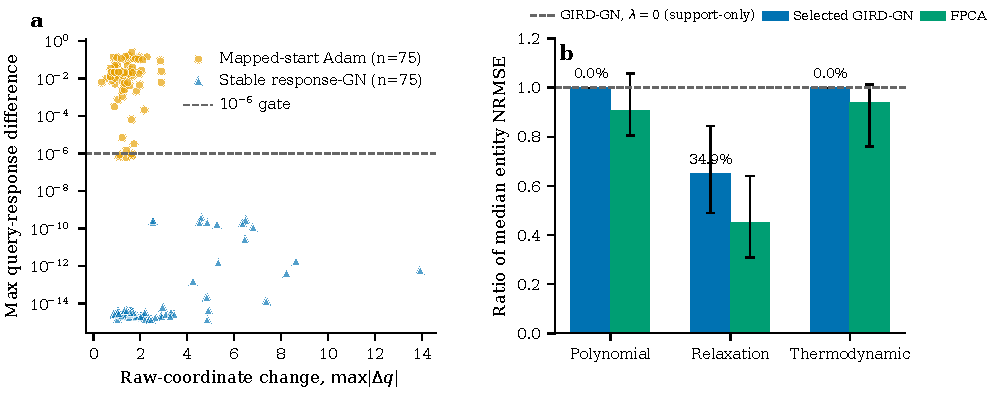
\includegraphics[width=0.90\textwidth]{figures/figure2_gauge_gird.pdf}
  \caption{Stable response-metric optimization preserves gauge-equivalent
  predictions, while GIRD gains are family-dependent in these controlled
  settings.  \textbf{(a)} Across 75 family--seed--gauge cases per method
  ($3$ families $\times5$ seeds $\times5$ gauges), raw coordinates move, but
  stable response-metric Gauss--Newton keeps the maximum query-response
  difference below $3.66\times10^{-10}$ (dashed pre-specified $10^{-6}$
  numerical tolerance), whereas
  mapped-start Adam reaches $0.255$.  \textbf{(b)} With four support points,
  GIRD-GN reduces median entity NRMSE only for relaxation
  ($0.0528\rightarrow0.0344$, $34.9\%$) and matches its $\lambda=0$ result for
  polynomial and thermodynamic charts.  FPCA has lower median NRMSE in all
  three tested families.  Bars are ratios of each method's median entity NRMSE
  to the support-only GIRD-GN $\lambda=0$ median; lower is better, and error
  bars are paired entity-bootstrap 95\% intervals (10,000 resamples) after
  five-seed pointwise aggregation.  Hyperparameters use fixed outer-training
  validation; outer-test queries are untouched.}
  \label{fig:gauge-gird}
\end{figure*}
